\documentclass[aspectratio=169, 10pt, t]{beamer}

% Hỗ trợ tiếng Việt tương thích XeLaTeX
\usepackage{iftex}
\ifXeTeX
  \usepackage{fontspec}
  \setmainfont{Arial}
  \setsansfont{Arial}
\else
  \usepackage[utf8]{inputenc}
  \usepackage[T5,T1]{fontenc}
  \usepackage{lmodern}
\fi

\usepackage{amsmath, amsfonts, amssymb}
\usepackage{graphicx}
\usepackage{booktabs}
\usepackage{tikz}
\usetikzlibrary{arrows.meta, positioning, shapes.geometric, calc}
\usepackage{tcolorbox}
\tcbuselibrary{skins}
\usepackage{hyperref}
\usepackage{ragged2e}

% Tinh chỉnh khoảng cách công thức toán
\setlength{\abovedisplayskip}{2pt}
\setlength{\belowdisplayskip}{2pt}
\setlength{\abovedisplayshortskip}{1pt}
\setlength{\belowdisplayshortskip}{1pt}

% ==================== BẢNG MÀU CAO CẤP (PREMIUM TECH PALETTE) ====================
\definecolor{CanvasBg}{RGB}{248, 250, 252}      % #F8FAFC - Nền xám ngọc công nghệ, làm nổi bật các thẻ trắng
\definecolor{MidnightNavy}{RGB}{15, 23, 42}     % #0F172A - Tiêu đề chính đậm, uy quyền
\definecolor{ElectricBlue}{RGB}{29, 78, 216}    % #1D4ED8 - Xanh dương hiện đại
\definecolor{TealAccent}{RGB}{13, 148, 136}     % #0D9488 - Xanh ngọc kỹ thuật
\definecolor{DeepPurple}{RGB}{99, 102, 241}     % #6366F1 - Tím xanh sang trọng
\definecolor{EmeraldGreen}{RGB}{16, 185, 129}   % #10B981 - Màu ảnh thật / Thành công
\definecolor{CrimsonCoral}{RGB}{225, 29, 72}    % #E11D48 - Màu ảnh AI / Cảnh báo
\definecolor{SlateBody}{RGB}{51, 65, 85}        % #334155 - Chữ nội dung sắc nét
\definecolor{SlateSub}{RGB}{100, 116, 139}      % #64748B - Chú thích và nhãn phụ
\definecolor{SlateBorder}{RGB}{226, 232, 240}   % #E2E8F0 - Viền thẻ mỏng tinh xảo
\definecolor{CardHeaderBg}{RGB}{241, 245, 249}  % #F1F5F9 - Nền header của thẻ

\usetheme{default}
\usecolortheme{dove}

\setbeamercolor{background canvas}{bg=CanvasBg}
\setbeamercolor{normal text}{fg=SlateBody}
\setbeamercolor{structure}{fg=MidnightNavy}
\setbeamercolor{item}{fg=ElectricBlue}
\setbeamercolor{subitem}{fg=TealAccent}

% Thiết lập căn trái chuẩn mực
\apptocmd{\frame}{}{\justifying}{}
\raggedright

% Bullet điểm nhấn hiện đại
\setbeamertemplate{itemize item}{\raise1.0pt\hbox{\textcolor{ElectricBlue}{\tiny$\blacksquare$}}}
\setbeamertemplate{itemize subitem}{\raise0.8pt\hbox{\textcolor{TealAccent}{\tiny$\bullet$}}}
\setbeamertemplate{navigation symbols}{}

% ==================== HEADER TỌA ĐỘ TUYỆT ĐỐI (100% KHÔNG BAO GIỜ LỆCH) ====================
\setbeamertemplate{headline}{}
\setbeamertemplate{frametitle}{
  \nointerlineskip
  \begin{tikzpicture}[remember picture, overlay]
    \node[anchor=north west, inner sep=0pt] at (current page.north west) {
      \begin{minipage}[t][1.30cm]{\paperwidth}
        \vspace{0.22cm}
        \hspace{0.85cm}
        \begin{minipage}{\dimexpr\paperwidth-1.7cm\relax}
          \raggedright
          \ifx\insertframesubtitle\@empty
            {\fontsize{7}{8.5}\selectfont\textbf{\textcolor{ElectricBlue}{\uppercase{Phương pháp nghiên cứu \;\textbar\; ZED Methodology}}}}\\[0.15em]
          \else
            {\fontsize{7}{8.5}\selectfont\textbf{\textcolor{ElectricBlue}{\uppercase{\insertframesubtitle}}}}\\[0.15em]
          \fi
          {\fontsize{13}{15.5}\selectfont\textbf{\textcolor{MidnightNavy}{\insertframetitle}}}
        \end{minipage}
      \end{minipage}
    };
    \draw[SlateBorder, line width=0.7pt] ($(current page.north west)+(0, -1.30cm)$) -- ($(current page.north east)+(0, -1.30cm)$);
  \end{tikzpicture}
  \vspace{1.15cm}
}

% ==================== FOOTER TỌA ĐỘ TUYỆT ĐỐI (100% CÂN XỨNG TOÀN TRANG) ====================
\setbeamertemplate{footline}{
  \begin{tikzpicture}[remember picture, overlay]
    \draw[SlateBorder, line width=0.5pt] ($(current page.south west)+(0, 0.65cm)$) -- ($(current page.south east)+(0, 0.65cm)$);
    \node[anchor=south west, inner sep=0pt] at ($(current page.south west)+(0.85cm, 0.18cm)$) {
      \tiny\textbf{\textcolor{MidnightNavy}{ZED: Zero-Shot Detection of AI-Generated Images}} \;\textcolor{SlateSub!60}{\textbar}\; \textcolor{SlateSub}{Cozzolino et al. (ECCV 2024)}
    };
    \node[anchor=south east, inner sep=0pt] at ($(current page.south east)+(-0.85cm, 0.15cm)$) {
      \tcbox[enhanced,colback=white,colframe=SlateBorder,boxrule=0.4pt,arc=1.0mm,top=0.15mm,bottom=0.15mm,left=1.6mm,right=1.6mm]{%
        \tiny\textbf{\textcolor{ElectricBlue}{\insertframenumber}} \textcolor{SlateSub!60}{/ \inserttotalframenumber}%
      }
    };
  \end{tikzpicture}
  \vspace{0.65cm}
}

% ==================== BỘ CARD UI CHUẨN MỰC (EQUAL HEIGHT SUPPORT) ====================
% 1. Standard Box: Nền trắng, header xám nhẹ, hỗ trợ equal height group
\newtcolorbox{cleanbox}[2][]{
  enhanced,
  colback=white,
  colframe=SlateBorder,
  colbacktitle=CardHeaderBg,
  coltitle=MidnightNavy,
  fonttitle=\bfseries\scriptsize,
  title=\ifstrempty{#2}{}{#2},
  boxrule=0.5pt,
  arc=2.0mm,
  titlerule=0.4pt,
  titlerule style={draw=SlateBorder},
  top=1.2mm, bottom=1.2mm, left=2.5mm, right=2.5mm,
  toptitle=0.8mm, bottomtitle=0.8mm,
  halign=left,
  #1
}

% 2. Accent Box: Nền trắng, vạch màu trên đỉnh (borderline north)
\newtcolorbox{accentbox}[3][]{
  enhanced,
  colback=white,
  colframe=SlateBorder,
  colbacktitle=CardHeaderBg,
  coltitle=#2,
  fonttitle=\bfseries\scriptsize,
  title=\ifstrempty{#3}{}{#3},
  boxrule=0.5pt,
  arc=2.0mm,
  titlerule=0.4pt,
  titlerule style={draw=SlateBorder},
  borderline north={2.2pt}{0pt}{#2},
  top=1.2mm, bottom=1.2mm, left=2.5mm, right=2.5mm,
  toptitle=0.8mm, bottomtitle=0.8mm,
  halign=left,
  #1
}

% 3. KPI Stat Box
\newtcolorbox{statbox}[3][]{
  enhanced,
  colback=white,
  colframe=SlateBorder,
  boxrule=0.5pt,
  arc=2.0mm,
  top=1.0mm, bottom=1.0mm, left=1.5mm, right=1.5mm,
  halign=center,
  borderline north={2.2pt}{0pt}{#2},
  #1
}

% 4. Note Box phẳng
\newtcolorbox{notebox}[1][]{
  enhanced,
  colback=white,
  colframe=SlateBorder,
  boxrule=0.4pt,
  arc=1.5mm,
  top=0.6mm, bottom=0.6mm, left=1.8mm, right=1.8mm,
  halign=left,
  #1
}

\begin{document}

% ==================== SLIDE 1: TRANG TIÊU ĐỀ ====================
\begin{frame}[plain]
  \vspace{0.8em}
  \begin{center}
    % Badge hội nghị
    \tcbox[enhanced,colback=ElectricBlue!8,colframe=ElectricBlue!35,boxrule=0.5pt,arc=3mm,top=0.9mm,bottom=0.9mm,left=4.0mm,right=4.0mm]{%
      \scriptsize\textbf{\textcolor{ElectricBlue}{ECCV 2024 \;\textbar\; BÁO CÁO CHUYÊN ĐỀ XỬ LÝ ẢNH NÂNG CAO}}%
    }
    
    \vspace{0.7em}
    {\fontsize{19}{23}\selectfont\textbf{\textcolor{MidnightNavy}{Phát hiện ảnh do AI sinh theo phương pháp Zero-Shot}}}
    
    \vspace{0.30em}
    {\fontsize{12.5}{15}\selectfont\textbf{\textcolor{ElectricBlue}{ZED: Zero-Shot Detection of AI-Generated Images}}}
    
    \vspace{0.45em}
    
\begin{tikzpicture}
      \fill[ElectricBlue] (0, 0) rectangle (2.5cm, 2.0pt);
      \fill[SlateBorder] (2.5cm, 0.5pt) rectangle (8.5cm, 1.5pt);
    \end{tikzpicture}
    
    \vspace{0.8em}
    \begin{minipage}{0.88\textwidth}
      \begin{tcolorbox}[enhanced,colback=white,colframe=SlateBorder,boxrule=0.5pt,arc=2.5mm,top=2.2mm,bottom=2.2mm,left=4.0mm,right=4.0mm]
        \begin{columns}[c]
          \begin{column}{0.48\textwidth}
            \raggedright\scriptsize
            \textbf{\textcolor{MidnightNavy}{Tác giả bài báo gốc:}}\\
            \textcolor{SlateBody}{Diego Cozzolino, Giovanni Poggi, Luisa Verdoliva}\\
            \textcolor{SlateSub}{\textit{Đại học Federico II Napoli, Ý --- ECCV 2024}}
          \end{column}
          \begin{column}{0.48\textwidth}
            \raggedright\scriptsize
            \textbf{\textcolor{MidnightNavy}{Trọng tâm chuyên đề báo cáo:}}\\
            \textcolor{SlateBody}{Nguyên lý nén Lossless, Phương pháp ZED,}\\
            \textcolor{SlateBody}{Pipeline thực thi \& Thực nghiệm 179,042 ảnh}
          \end{column}
        \end{columns}
      \end{tcolorbox}
    \end{minipage}
  \end{center}
\end{frame}

% ==================== SLIDE 2: MỤC LỤC BÁO CÁO (GRID 2x2 CÂN XỨNG HOÀN TOÀN) ====================
\begin{frame}{Nội dung báo cáo}
  \framesubtitle{TỔNG QUAN LỘ TRÌNH \;\textbar\; PRESENTATION ROADMAP}
  \begin{columns}[t]
    \begin{column}{0.48\textwidth}
      \begin{accentbox}[equal height group=toc1, top=0.7mm, bottom=0.7mm]{ElectricBlue}{01. Phương pháp nghiên cứu ZED}
        \raggedright\scriptsize
        \textbf{3.1 Bối cảnh:} Khởi nguồn từ next-token prediction \& NLL.\\
        \vspace{0.04em}
        \textbf{3.2 Tiếp cận thị giác:} Chuyển sang bài toán one-class.\\
        \vspace{0.04em}
        \textbf{3.3 Quy trình tổng thể:} Sơ đồ trích xuất đặc trưng đa tầng.\\
        \vspace{0.04em}
        \textbf{3.4 Cơ sở toán học:} Discretized logistic mixture, NLL \& entropy.
      \end{accentbox}
      \vspace{0.05em}
      \begin{accentbox}[equal height group=toc2, top=0.7mm, bottom=0.7mm]{TealAccent}{02. Quy trình thực thi hai giai đoạn}
        \raggedright\scriptsize
        Phân định rành mạch 2 giai đoạn: \textbf{Phase 1 Training} (huấn luyện bộ nén lossless trên ảnh thật) $\longrightarrow$ \textbf{Phase 2 Zero-shot Detection} (tính anomaly score và so sánh ngưỡng).
      \end{accentbox}
    \end{column}
    \begin{column}{0.48\textwidth}
      \begin{accentbox}[equal height group=toc1, top=0.7mm, bottom=0.7mm]{DeepPurple}{03. Thực nghiệm của Paper gốc (ECCV 2024)}
        \raggedright\scriptsize
        \textbf{5.1 Thiết lập benchmark:} Open Images (338k ảnh thật, 0 ảnh AI), tập kiểm thử 29k ảnh AI từ hơn 20 mô hình sinh.\\
        \vspace{0.04em}
        \textbf{5.2 So sánh SoTA:} Vượt trội các mô hình giám sát khi gặp generator mới, đạt AUC $>90\text{--}95\%$, $+3.4\%$ accuracy.
      \end{accentbox}
      \vspace{0.05em}
      \begin{accentbox}[equal height group=toc2, top=0.7mm, bottom=0.7mm]{MidnightNavy}{04. Thực nghiệm độc lập \& Đánh giá 70/30}
        \raggedright\scriptsize
        \textbf{6.1 Huấn luyện:} 32 epochs (~29h GPU), loss giảm 58.27 $\to$ 29.20.\\
        \vspace{0.04em}
        \textbf{6.2 Kiểm định 179,042 ảnh:} Phân tầng 70\% Calib $\to$ 30\% Test ngoài mẫu; $|D^{(0)}|$ đạt 68.76\% AUC, 64.01\% Balanced Acc.
      \end{accentbox}
    \end{column}
  \end{columns}
\end{frame}

% ==================== SLIDE 3: 3.1 BỐI CẢNH ====================
\begin{frame}{3.1 Bối cảnh: Khởi nguồn từ phát hiện văn bản do LLM sinh}
  \framesubtitle{PHƯƠNG PHÁP NGHIÊN CỨU \;\textbar\; ZED METHODOLOGY}
  \begin{columns}[t]
    \begin{column}{0.50\textwidth}
      \begin{accentbox}[equal height group=ctx]{ElectricBlue}{Nguyên lý phát hiện văn bản máy sinh}
        \raggedright\scriptsize
        \textbf{1. Mô hình autoregressive:}\\
        Các mô hình ngôn ngữ lớn (LLM) sinh chuỗi token tuần tự theo xác suất có điều kiện từng bước.
        \vspace{0.30em}

        \textbf{2. Mức độ bất ngờ (surprisal):}\\
        Văn bản máy sinh ưu tiên token có xác suất cao nhất (greedy / top-$p$); văn bản con người chứa nhiều biến thiên phong phú.
        \vspace{0.30em}

        \textbf{3. Định lượng qua NLL:}\\
        Mức độ bất ngờ tích lũy trên chuỗi được đo bằng Negative Log-Likelihood (NLL).
      \end{accentbox}
    \end{column}
    \begin{column}{0.50\textwidth}
      \begin{accentbox}[equal height group=ctx]{TealAccent}{Quy luật phân tách thống kê}
        \raggedright\scriptsize
        \textbf{1. Văn bản do AI sinh:}\\
        Tổng NLL rất thấp và phân bố tập trung do mô hình tự tin dự đoán các token quen thuộc.
        \vspace{0.35em}

        \textbf{2. Văn bản do người viết:}\\
        Tổng NLL cao hơn rõ rệt và phân bố rộng khắp trên không gian thống kê.
        \vspace{0.35em}

        $\blacktriangleright$ Sự chênh lệch NLL này tạo nên ranh giới rõ rệt để phân loại văn bản máy sinh và văn bản người viết.
      \end{accentbox}
    \end{column}
  \end{columns}
\end{frame}

% ==================== SLIDE 4: 3.1 CƠ CHẾ TOÁN HỌC ====================
\begin{frame}{3.1 Next-Token Prediction và Negative Log-Likelihood}
  \framesubtitle{PHƯƠNG PHÁP NGHIÊN CỨU \;\textbar\; ZED METHODOLOGY}
  \begin{cleanbox}{Biểu diễn toán học Next-Token Prediction}
    \raggedright\scriptsize
    Ánh xạ chuỗi văn bản $s$ thành chuỗi token $T(s) = \{x_0, x_1, \dots, x_L\}$. Xác suất đồng thời phân rã chuỗi:
    \\[0.15em]
    \centering
    $\textstyle P(s) = \prod_{i=1}^L P(x_i \mid x_0, \dots, x_{i-1}) = \prod_{i=1}^L P(x_i \mid X_i) \quad \text{với } X_i = \{x_0, \dots, x_{i-1}\}$
  \end{cleanbox}

  \vspace{0.15em}
  \begin{columns}[t]
    \begin{column}{0.50\textwidth}
      \begin{accentbox}[equal height group=math]{ElectricBlue}{Negative Log-Likelihood (NLL)}
        \raggedright\scriptsize
        Độ bất ngờ (surprisal) tích lũy trên toàn bộ chuỗi được định lượng qua NLL:
        \\[0.20em]
        \centering
        $\textstyle \text{NLL}(s) = -\sum_{i=1}^L \log P(x_i \mid X_i)$
        \vspace{0.15em}
        \raggedright
        Giá trị NLL càng nhỏ thể hiện chuỗi càng quen thuộc và dễ dự đoán đối với mô hình.
      \end{accentbox}
    \end{column}
    \begin{column}{0.50\textwidth}
      \begin{accentbox}[equal height group=math]{TealAccent}{Đặc trưng phân tách hai miền}
        \raggedright\scriptsize
        \textbf{Machine-generated text:} NLL thấp và phân tán hẹp do mô hình tự tin cao trong từng bước sinh.
        \vspace{0.25em}

        \textbf{Human-written text:} NLL cao hơn và phân tán rộng khắp.
        \vspace{0.25em}

        $\blacktriangleright$ Đây chính là tiền đề lý thuyết để chuyển giao sang thị giác máy tính 2D.
      \end{accentbox}
    \end{column}
  \end{columns}
\end{frame}

% ==================== SLIDE 5: 3.2 TỪ VĂN BẢN SANG HÌNH ẢNH ====================
\begin{frame}{3.2 Từ văn bản sang hình ảnh: Bài toán one-class}
  \framesubtitle{PHƯƠNG PHÁP NGHIÊN CỨU \;\textbar\; ZED METHODOLOGY}
  \begin{columns}[T, totalwidth=\linewidth]
    \begin{column}{0.50\linewidth}
      \begin{accentbox}[equal height group=s5box, top=0.5mm, bottom=0.5mm]{CrimsonCoral}{Thách thức khi mở rộng sang ảnh 2D}
        \raggedright\tiny
        \textbf{1. Lưới pixel 2D:}\\
        Thứ tự quét tuần tự (raster-scan) phá vỡ tương quan không gian đa hướng.\\
        \vspace{0.05em}
        \textbf{2. Cơ chế sinh khác biệt:}\\
        Mô hình Diffusion/GAN không sinh token tuần tự mà khử nhiễu song song.\\
        \vspace{0.05em}
        \textbf{3. Không gian liên tục:}\\
        Không gian RGB đa chiều phức tạp hơn nhiều so với từ vựng rời rạc.
      \end{accentbox}
      \vspace{0.06em}
      \begin{accentbox}[equal height group=s5box, top=0.5mm, bottom=0.5mm]{EmeraldGreen}{Định hướng tiếp cận one-class}
        \raggedright\tiny
        \textbf{1. Đổi hệ quy chiếu:}\\
        Không chạy theo từng công cụ sinh; học phân phối chuẩn của \textbf{ảnh tự nhiên} $P_{\text{real}}(x)$.\\
        \vspace{0.05em}
        \textbf{2. Coi ảnh AI là mẫu dị biệt:}\\
        Xem mọi ảnh máy sinh là mẫu ngoại lai (anomaly/outlier) so với ảnh thật.\\
        \vspace{0.05em}
        \textbf{3. Nhận diện zero-shot:}\\
        Mô hình hóa chính xác ảnh thật là đủ để phát hiện mà không cần ảnh giả khi train.
      \end{accentbox}
    \end{column}
    \begin{column}{0.48\linewidth}
      \centering
      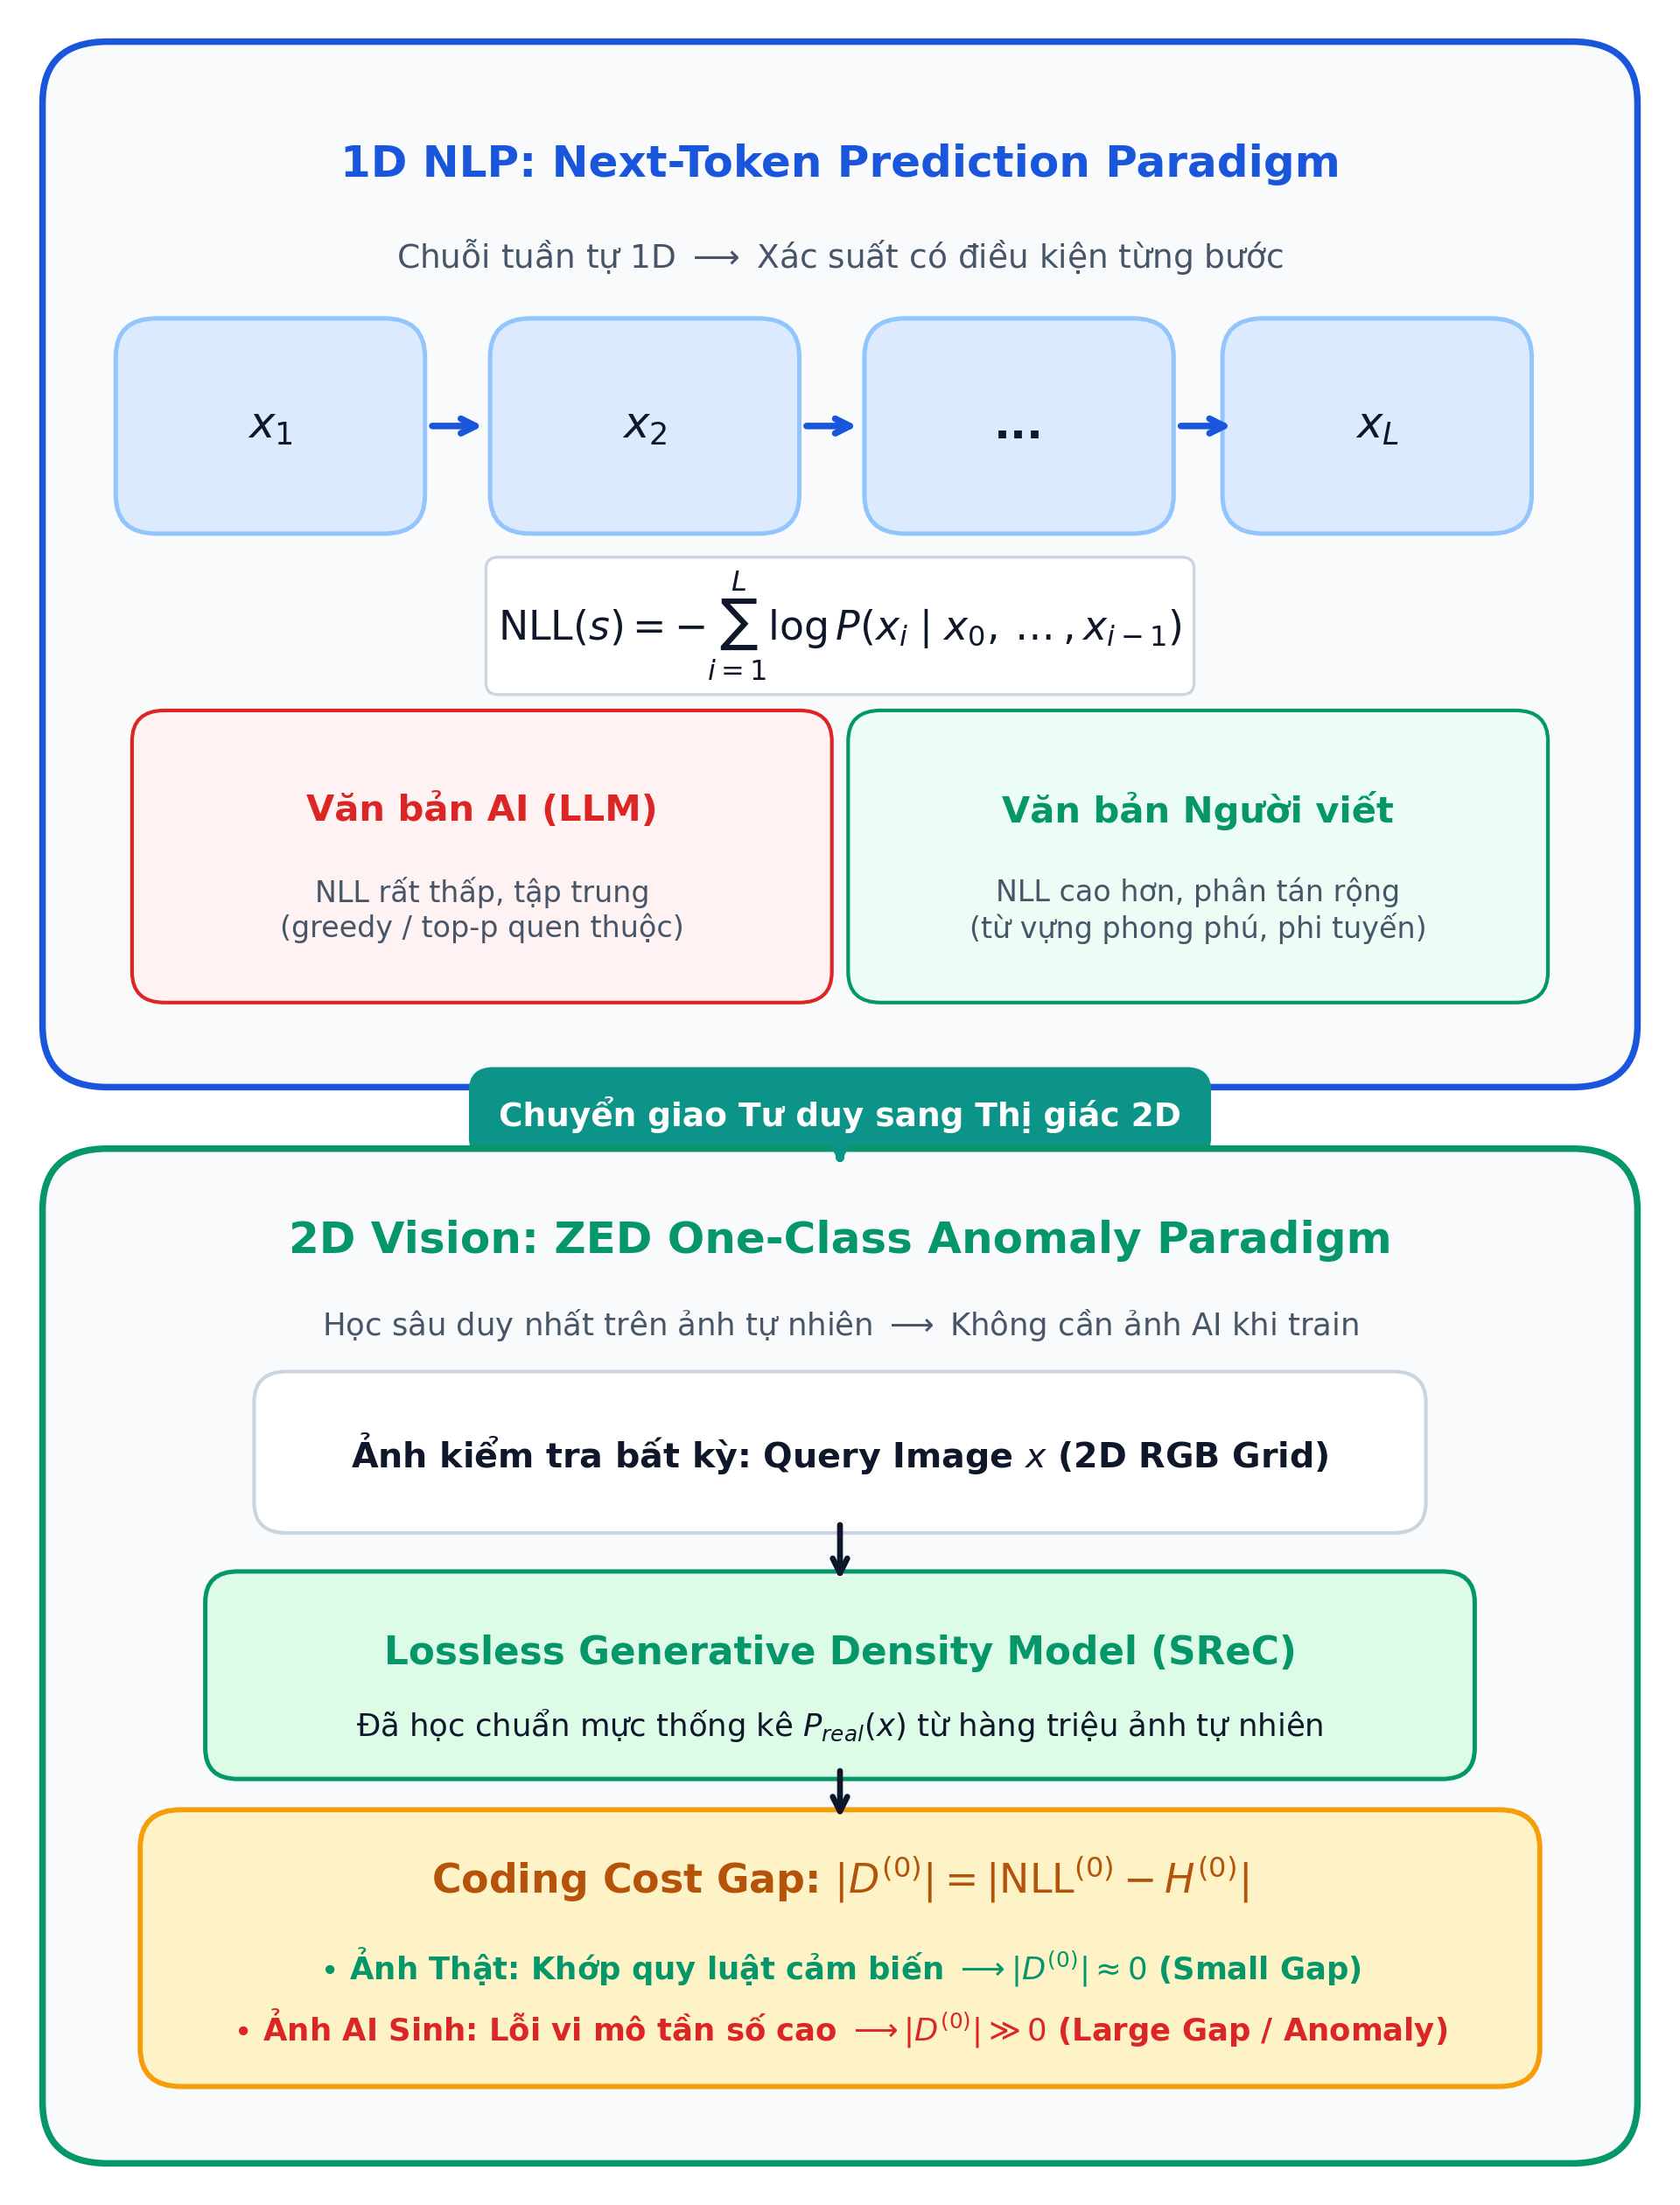
\includegraphics[width=\linewidth,height=0.50\textheight,keepaspectratio]{figures/fig_nlp_vs_vision_vert.png}\\[0.08em]
      \tiny\textcolor{SlateSub}{So sánh mô hình: Autoregressive 1D vs Khung nhận diện one-class 2D}
    \end{column}
  \end{columns}
\end{frame}

% ==================== SLIDE 6: 3.3 QUY TRÌNH TRÍCH XUẤT ĐẶC TRƯNG ====================
\begin{frame}{3.3 Sơ đồ quy trình trích xuất đặc trưng toàn diện}
  \framesubtitle{PHƯƠNG PHÁP NGHIÊN CỨU \;\textbar\; ZED METHODOLOGY}
  \centering
  \vspace{0.04cm}
  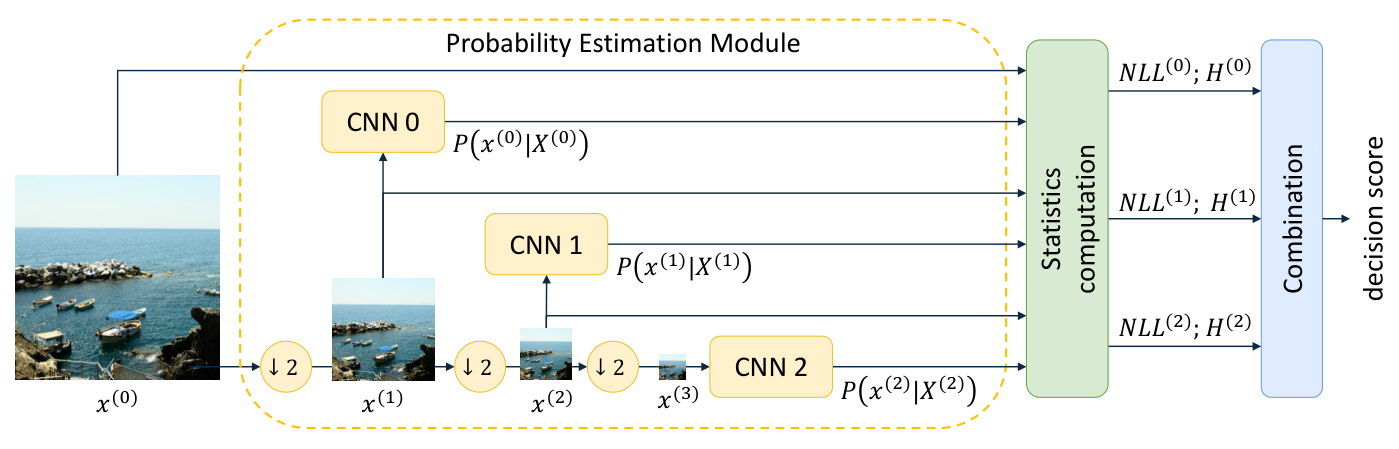
\includegraphics[width=0.92\linewidth,height=0.28\textheight,keepaspectratio]{figures/fig3_pipeline.png}\\[0.10em]
  \vspace{-0.10em}
  \begin{columns}[t]
    \begin{column}{0.50\textwidth}
      \begin{cleanbox}[equal height group=pipe, top=1.0mm, bottom=1.0mm]{Kim tự tháp đa phân giải (SReC Pyramid)}
        \raggedright\scriptsize
        \textbf{1. Giảm mẫu và làm tròn số nguyên:}\\
        Ảnh gốc $x^{(0)}$ qua average pooling $2\times2$ tạo ảnh $y^{(1)}$, làm tròn thành số nguyên $x^{(1)} = \text{round}(y^{(1)}) \in \{0, \dots, 255\}$. Lặp lại tạo 4 cấp phân giải $\{x^{(0)}, x^{(1)}, x^{(2)}, x^{(3)}\}$.\\
        \vspace{0.12em}
        \textbf{2. Tầng đáy $l=3$:}\\
        Ảnh thu nhỏ nhất ($H/8 \times W/8$), mã hóa trực tiếp không cần mạng neural.
      \end{cleanbox}
    \end{column}
    \begin{column}{0.50\textwidth}
      \begin{cleanbox}[equal height group=pipe, top=1.0mm, bottom=1.0mm]{Khối CNN ước lượng xác suất}
        \raggedright\scriptsize
        \textbf{1. Ba mạng CNN chuyên biệt:}\\
        Hoạt động tại các cấp phân giải $l=2, 1, 0$, nhận ngữ cảnh từ tầng dưới để dự đoán phân phối xác suất tầng trên.\\
        \vspace{0.12em}
        \textbf{2. Xử lý song song tốc độ cao:}\\
        Tại mỗi bước, các nhóm $2\times2$ sub-pixel trên toàn ảnh được CNN xử lý song song, loại bỏ độ trễ tuần tự.
      \end{cleanbox}
    \end{column}
  \end{columns}
\end{frame}

% ==================== SLIDE 7: 3.4 MÔ HÌNH HÓA XÁC SUẤT VÀ NLL ====================
\begin{frame}{3.4 Mô hình hóa xác suất điểm ảnh và tính toán NLL}
  \framesubtitle{PHƯƠNG PHÁP NGHIÊN CỨU \;\textbar\; ZED METHODOLOGY}
  \begin{columns}[T, totalwidth=\linewidth]
    \begin{column}{0.48\linewidth}
      \begin{cleanbox}[top=0.5mm, bottom=0.5mm]{Discretized Logistic Mixture ($K=10$)}
        \raggedright\tiny
        Mức xám $k \in \{0, \dots, 255\}$ tính xác suất bằng tích phân mật độ hỗn hợp logistic trên đoạn làm tròn $[k - 0.5, k + 0.5]$:
        \vspace{-0.25em}
        {\tiny
        \begin{equation*}
          \begin{aligned}
            P(x = k \mid X) = \sum_{m=1}^{10} w_m \cdot \Big[ & \sigma\left((k + 0.5 - \mu_m)/s_m\right) \\
            & - \sigma\left((k - 0.5 - \mu_m)/s_m\right) \Big]
          \end{aligned}
        \end{equation*}}
        \vspace{-0.35em}
        Mạng CNN nhận ngữ cảnh $X$ và xuất ra $3K = 30$ tham số $(w_m, \mu_m, s_m)$ cho mỗi điểm ảnh.
      \end{cleanbox}
      \vspace{0.08em}
      \begin{accentbox}[top=0.5mm, bottom=0.5mm]{ElectricBlue}{Bản đồ chi phí nén thực tế (NLL Map)}
        \raggedright\tiny
        $\bullet$ \textbf{Chi phí tại từng pixel:} $\text{NLL}^{(l)}_{i,j} = -\log_2 P(x^{(l)}_{i,j} \mid X^{(l)}_{i,j})$.\\
        \vspace{0.06em}
        $\bullet$ \textbf{Chi phí trung bình toàn ảnh:} $\text{NLL}^{(l)} = \frac{1}{NM} \sum_{i,j} \text{NLL}^{(l)}_{i,j}$.\\
        \vspace{0.06em}
        $\blacktriangleright$ Thể hiện số bit thực tế cần tiêu tốn để mã hóa điểm ảnh.
      \end{accentbox}
    \end{column}
    \begin{column}{0.50\linewidth}
      \centering
      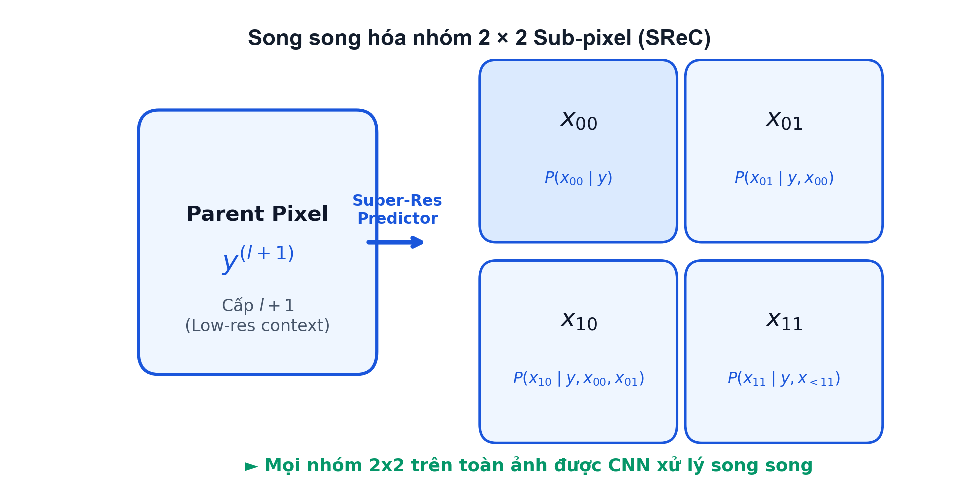
\includegraphics[width=\linewidth,height=0.36\textheight,keepaspectratio]{figures/fig_subpixel_srec.pdf}\\[0.08em]
      \tiny\textcolor{SlateSub}{Cơ chế dự đoán và xử lý song song nhóm $2 \times 2$ sub-pixel (SReC)}\\[0.15em]
      \begin{notebox}[top=0.6mm, bottom=0.6mm]
        \raggedright\tiny
        \textbf{Ưu thế tính toán của SReC:}\\
        Thay vì sinh tuần tự từng điểm ảnh như mô hình autoregressive 1D, SReC phân tách thành các nhóm $2 \times 2$ sub-pixel và xử lý song song toàn ảnh bằng CNN, loại bỏ nút thắt cổ chai về độ trễ suy luận.
      \end{notebox}
    \end{column}
  \end{columns}
\end{frame}

% ==================== SLIDE 8: 3.4 BẢN ĐỒ ENTROPY ====================
\begin{frame}{3.4 Bản đồ Entropy và kỳ vọng chi phí nén}
  \framesubtitle{PHƯƠNG PHÁP NGHIÊN CỨU \;\textbar\; ZED METHODOLOGY}
  \begin{columns}[T, totalwidth=\linewidth]
    \begin{column}{0.48\linewidth}
      \begin{cleanbox}[top=0.6mm, bottom=0.6mm]{Xác suất $P_k$ và bản đồ Entropy}
        \raggedright\tiny
        \textbf{1. Ý nghĩa của $P_k$:}\\
        $P_k = P(x^{(l)}_{i,j} = k \mid X^{(l)}_{i,j})$ là xác suất do CNN dự đoán cho pixel $(i, j)$ nhận mức xám thứ $k \in \{0, \dots, 255\}$.\\
        \vspace{0.10em}
        \textbf{2. Công thức Entropy tại từng pixel:}\\
        \centering
        $\textstyle H^{(l)}_{i,j} = -\sum_{k=0}^{255} P_k \log_2 P_k$\\[0.10em]
        \raggedright
        \textbf{3. Ý nghĩa vật lý:}\\
        Đo mức độ bất định. Đây là \textbf{kỳ vọng toán học} của độ dài mã nén nếu pixel thực sự tuân theo phân phối đã học.
      \end{cleanbox}
      \vspace{0.08em}
      \begin{accentbox}[top=0.6mm, bottom=0.6mm]{EmeraldGreen}{Entropy toàn ảnh \& Coding Cost Gap}
        \raggedright\tiny
        $\bullet$ \textbf{Entropy trung bình toàn ảnh:} $H^{(l)} = \frac{1}{NM} \sum_{i,j} H^{(l)}_{i,j}$.\\
        \vspace{0.06em}
        $\bullet$ \textbf{Khoảng cách chi phí ($D^{(l)}$):} $D^{(l)} = \text{NLL}^{(l)} - H^{(l)}$ đo độ lệch giữa chi phí thực tế và kỳ vọng Shannon.
      \end{accentbox}
    \end{column}
    \begin{column}{0.50\linewidth}
      \centering
      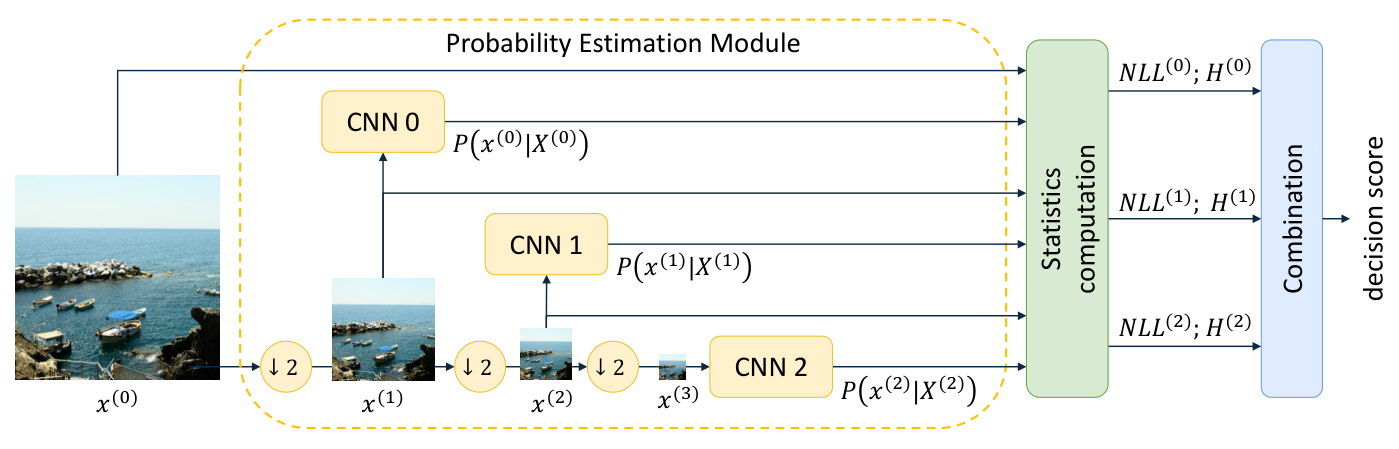
\includegraphics[width=\linewidth,height=0.30\textheight,keepaspectratio]{figures/fig3_pipeline.png}\\[0.10em]
      \tiny\textcolor{SlateSub}{Khối tính toán thống kê: Từ phân phối xác suất dự đoán $P(x \mid X) \to \text{NLL}$ và $H$}\\[0.15em]
      \begin{notebox}[top=0.6mm, bottom=0.6mm]
        \raggedright\tiny
        \textbf{Quy luật Shannon trong ZED:}\\
        $\bullet$ \textbf{Ảnh thật:} Chi phí thực tế khớp kỳ vọng: $\text{NLL}^{(l)} \approx H^{(l)} \longrightarrow D^{(l)} \approx 0$.\\
        $\bullet$ \textbf{Ảnh AI:} Vi phạm thống kê tự nhiên $\longrightarrow \text{NLL}^{(l)}$ lệch xa kỳ vọng $H^{(l)} \longrightarrow |D^{(l)}| \gg 0$.
      \end{notebox}
    \end{column}
  \end{columns}
\end{frame}

% ==================== SLIDE 9: 3.4 BẢN CHẤT VẬT LÝ ====================
\begin{frame}{3.4 Bản chất vật lý: Chi phí thực tế so với kỳ vọng}
  \framesubtitle{PHƯƠNG PHÁP NGHIÊN CỨU \;\textbar\; ZED METHODOLOGY}
  \centering
  \vspace{0.04cm}
  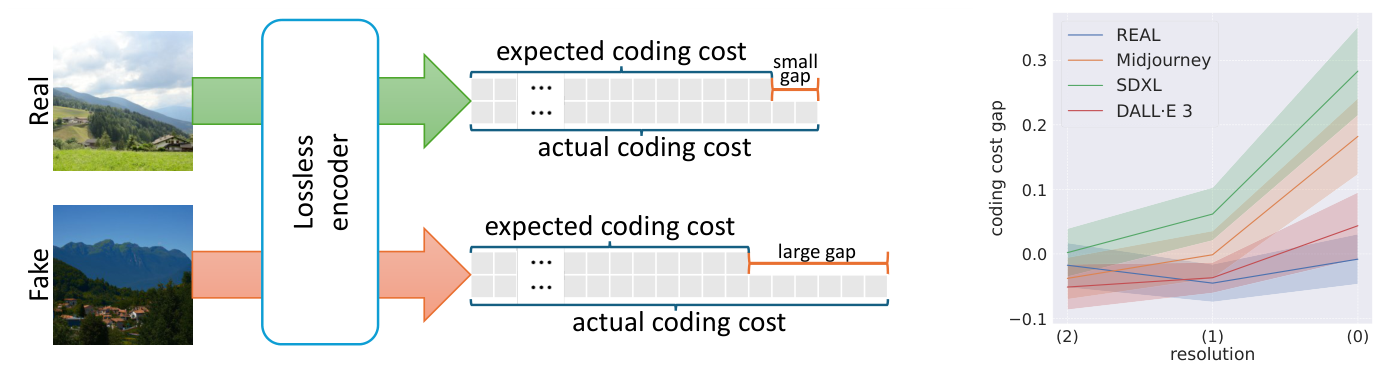
\includegraphics[width=0.92\linewidth,height=0.30\textheight,keepaspectratio]{figures/fig1_teaser.png}\\[0.10em]
  \vspace{-0.10em}
  \begin{columns}[t]
    \begin{column}{0.50\textwidth}
      \begin{accentbox}[equal height group=phys, top=1.0mm, bottom=1.0mm]{EmeraldGreen}{Ảnh thật tự nhiên}
        \raggedright\scriptsize
        Phân phối pixel khớp hoàn hảo tri thức bộ mã hóa. Chi phí mã hóa thực tế xấp xỉ kỳ vọng: $\text{NLL}^{(l)} \approx H^{(l)}$ ở tất cả mọi cấp độ phân giải $l \in \{0, 1, 2\}$.
      \end{accentbox}
    \end{column}
    \begin{column}{0.50\textwidth}
      \begin{accentbox}[equal height group=phys, top=1.0mm, bottom=1.0mm]{CrimsonCoral}{Ảnh do AI sinh}
        \raggedright\scriptsize
        Ngữ nghĩa vĩ mô ($l=2, 1$) bình thường, nhưng tại phân giải gốc ($l=0$) thiếu hụt tính ngẫu nhiên vi mô của cảm biến thực. Hệ quả: $\text{NLL}^{(0)}$ lệch xa kỳ vọng $H^{(0)}$ (lệch dương hoặc lệch âm sâu).
      \end{accentbox}
    \end{column}
  \end{columns}
\end{frame}

% ==================== SLIDE 10: 3.4 SO SÁNH BẢN ĐỒ KHÔNG GIAN ====================
\begin{frame}{3.4 Bản đồ không gian: So sánh trực quan NLL và Entropy}
  \framesubtitle{PHƯƠNG PHÁP NGHIÊN CỨU \;\textbar\; ZED METHODOLOGY}
  \centering
  \vspace{0.04cm}
  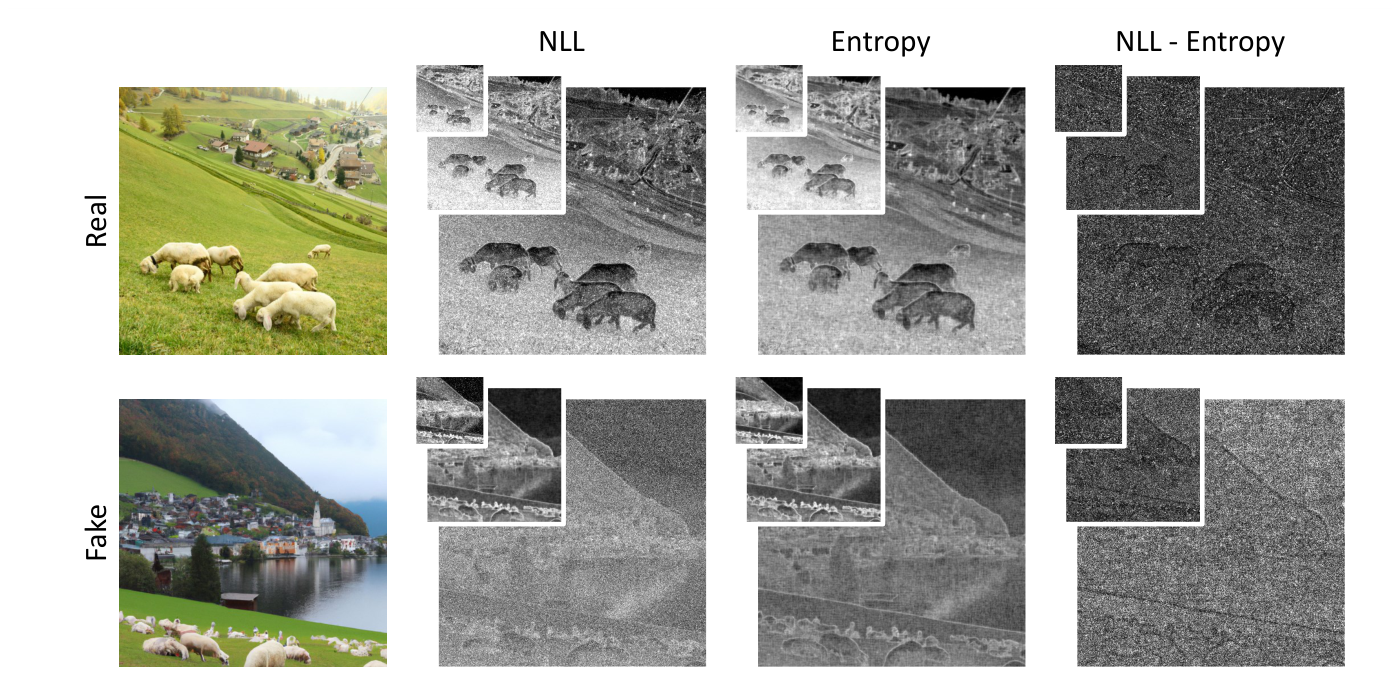
\includegraphics[width=0.92\linewidth,height=0.30\textheight,keepaspectratio]{figures/fig2_nll_entropy.png}\\[0.10em]
  \vspace{-0.10em}
  \begin{columns}[t]
    \begin{column}{0.50\textwidth}
      \begin{accentbox}[equal height group=spat, top=1.0mm, bottom=1.0mm]{EmeraldGreen}{Hàng trên: Ảnh thật tự nhiên}
        \raggedright\scriptsize
        Bản đồ hiệu số $\text{NLL}^{(0)} - H^{(0)}$ tối đen đồng đều vì chi phí thực tế và kỳ vọng xấp xỉ bằng nhau trên mọi vị trí điểm ảnh.
      \end{accentbox}
    \end{column}
    \begin{column}{0.50\textwidth}
      \begin{accentbox}[equal height group=spat, top=1.0mm, bottom=1.0mm]{CrimsonCoral}{Hàng dưới: Ảnh do AI sinh}
        \raggedright\scriptsize
        Bản đồ hiệu số $\text{NLL}^{(0)} - H^{(0)}$ sáng rực trên khắp bề mặt, bộc lộ rõ rệt sự bất thường thống kê ở cấu trúc vi mô do AI tạo ra.
      \end{accentbox}
    \end{column}
  \end{columns}
\end{frame}

% ==================== SLIDE 11: 3.4 THỐNG KÊ QUYẾT ĐỊNH ====================
\begin{frame}{3.4 Khoảng cách chi phí nén và thống kê quyết định}
  \framesubtitle{PHƯƠNG PHÁP NGHIÊN CỨU \;\textbar\; ZED METHODOLOGY}
  \centering
  \vspace{0.04cm}
  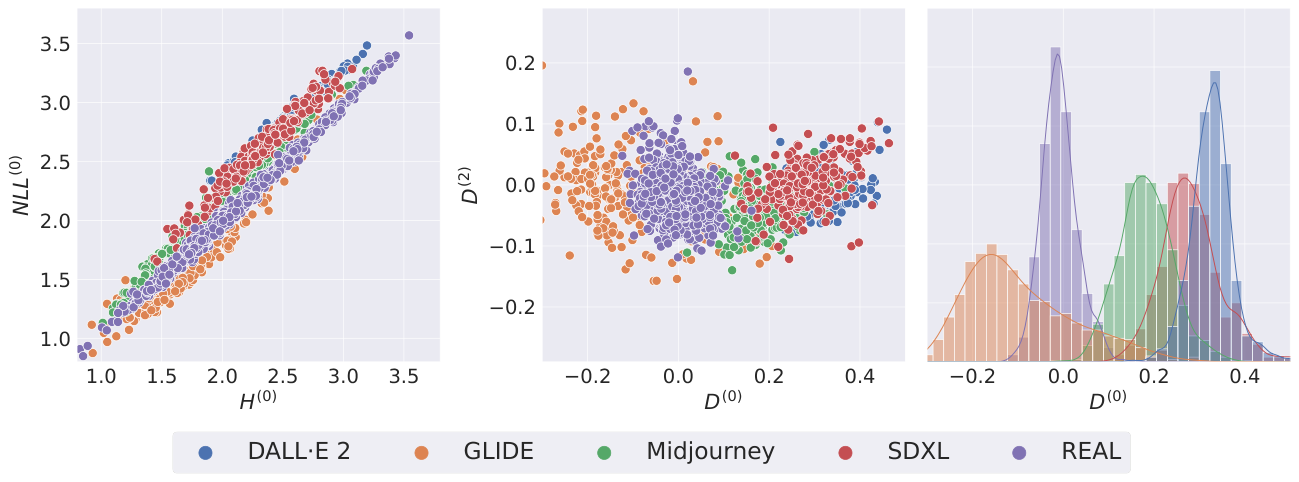
\includegraphics[width=0.92\linewidth,height=0.30\textheight,keepaspectratio]{figures/fig5_decision_stats.png}\\[0.10em]
  \vspace{-0.10em}
  \begin{columns}[t]
    \begin{column}{0.33\textwidth}
      \begin{cleanbox}[equal height group=dec, top=1.0mm, bottom=1.0mm]{Khoảng cách chi phí}
        \raggedright\scriptsize
        $D^{(l)} = \text{NLL}^{(l)} - H^{(l)}$\\
        đo độ lệch giữa chi phí thực tế và kỳ vọng của bộ mã hóa.
      \end{cleanbox}
    \end{column}
    \begin{column}{0.34\textwidth}
      \begin{cleanbox}[equal height group=dec, top=1.0mm, bottom=1.0mm]{Các biến thể thống kê}
        \raggedright\scriptsize
        $\blacktriangleright$ $D^{(0)}$: Phân giải gốc vi mô.\\
        $\blacktriangleright$ $|D^{(0)}|$: Trị tuyệt đối độ lệch.\\
        $\blacktriangleright$ $|\Delta^{01}| = |D^{(0)} - D^{(1)}|$: Vi phân.
      \end{cleanbox}
    \end{column}
    \begin{column}{0.33\textwidth}
      \begin{cleanbox}[equal height group=dec, top=1.0mm, bottom=1.0mm]{Năng lực phân tách}
        \raggedright\scriptsize
        NLL hoặc H đơn lẻ bị chồng lấn; $|D^{(0)}|$ và $|\Delta^{01}|$ tách biệt rõ rệt phân phối thật và nhân tạo.
      \end{cleanbox}
    \end{column}
  \end{columns}
\end{frame}

% ==================== SLIDE 12: PIPELINE THỰC THI ====================
\begin{frame}{Quy trình thực thi ZED: Huấn luyện vs Nhận diện zero-shot}
  \framesubtitle{QUY TRÌNH THỰC THI THỰC TẾ \;\textbar\; OPERATIONAL PIPELINE}
  \begin{columns}[t]
    \begin{column}{0.50\textwidth}
      \begin{accentbox}[equal height group=pipeexec]{ElectricBlue}{Phase 1: Huấn luyện bộ nén (ảnh thật)}
        \raggedright\scriptsize
        \textbf{1. Dữ liệu đầu vào:}\\
        Chỉ dùng \textbf{ảnh tự nhiên thế giới thực} (One-Class setup). Tuyệt đối không nạp ảnh AI khi huấn luyện.
        \vspace{0.18em}

        \textbf{2. Học quy luật phân phối tự nhiên:}\\
        Mạng CNN học xác suất có điều kiện của điểm ảnh qua SReC và Discretized Logistic Mixture $K=10$.
        \vspace{0.18em}

        \textbf{3. Tối ưu hàm mất mát (MLE):}\\
        Tối thiểu hóa Cross Entropy / NLL trên tập ảnh thật, giúp mô hình nén ảnh thật với số bit tối ưu theo định lý Shannon ($\text{NLL} \approx H$).
        \vspace{0.18em}

        \textbf{4. Đóng băng mô hình:}\\
        Trọng số được \textbf{đóng băng vĩnh viễn}, thiết lập một chuẩn mực entropy kỳ vọng $H^{(0)}$ bất biến.
      \end{accentbox}
    \end{column}
    \begin{column}{0.50\textwidth}
      \begin{accentbox}[equal height group=pipeexec]{TealAccent}{Phase 2: Nhận diện zero-shot (Anomaly scoring)}
        \raggedright\scriptsize
        \textbf{1. Dữ liệu kiểm tra:}\\
        Ảnh kiểm tra bất kỳ (không nhãn, không phụ thuộc kiến trúc bộ sinh tạo ra ảnh).
        \vspace{0.18em}

        \textbf{2. Trích xuất chỉ số qua mô hình đóng băng:}\\
        $\bullet$ Tính chi phí thực tế $\text{NLL}^{(0)}$ và kỳ vọng $H^{(0)}$.\\
        $\bullet$ Tính khoảng cách chi phí: $|D^{(0)}| = |\text{NLL}^{(0)} - H^{(0)}|$ và $|\Delta^{01}|$.
        \vspace{0.18em}

        \textbf{3. So sánh ngưỡng quyết định $\tau^*$:}\\
        $\bullet$ Điểm quyết định $> \tau^* \longrightarrow$ \textbf{\textcolor{CrimsonCoral}{Dự đoán: Ảnh do AI sinh}}.\\
        $\bullet$ Điểm quyết định $\le \tau^* \longrightarrow$ \textbf{\textcolor{EmeraldGreen}{Dự đoán: Ảnh thật tự nhiên}}.
        \vspace{0.18em}

        \textbf{4. Khả năng zero-shot:}\\
        Nhận diện lập tức các bộ sinh hoàn toàn mới lạ mà không cần tái huấn luyện.
      \end{accentbox}
    \end{column}
  \end{columns}
\end{frame}

% ==================== SLIDE 13: 5.1 THỰC NGHIỆM PAPER GỐC: DATASETS ====================
\begin{frame}{5.1 Thực nghiệm paper gốc: Dữ liệu huấn luyện \& Benchmark}
  \framesubtitle{THỰC NGHIỆM PAPER GỐC \;\textbar\; ORIGINAL PAPER EVALUATION}
  \begin{columns}[t, totalwidth=\linewidth]
    \begin{column}{0.48\linewidth}
      \begin{cleanbox}[equal height group=origexp, top=0.8mm, bottom=0.8mm]{Thiết lập huấn luyện (Training Set)}
        \raggedright\scriptsize
        $\bullet$ \textbf{Khung tiếp cận One-Class (Real-only):}\\
        Chỉ học trên ảnh tự nhiên, \textbf{hoàn toàn không có ảnh AI}.
        \vspace{0.18em}

        $\bullet$ \textbf{Tập dữ liệu huấn luyện chính:}\\
        \textbf{Open Images dataset} ($\approx$338,000 ảnh chất lượng cao).
        \vspace{0.18em}

        $\bullet$ \textbf{Các tập dữ liệu khảo sát đối chiếu:}\\
        Huấn luyện đối sánh độc lập trên \textbf{LAION} ($\approx$117k ảnh) và \textbf{MS-COCO} ($\approx$106k ảnh).
        \vspace{0.18em}

        $\bullet$ \textbf{Kiểm định không bị ảnh hưởng nén JPEG:}\\
        Bổ sung biến thể nén JPEG ngẫu nhiên (Quality 80--100) để chứng minh bộ nén không bị lệ thuộc vào định dạng nén.
        \vspace{0.18em}

        $\bullet$ \textbf{Cấu hình:}\\
        SReC 3 cấp độ phân giải subpixel ($L=3$), mô hình Discretized Logistic Mixture ($K=10$), tối ưu hóa NLL.
      \end{cleanbox}
    \end{column}
    \begin{column}{0.50\linewidth}
      \begin{accentbox}[equal height group=origexp, top=0.8mm, bottom=0.8mm]{ElectricBlue}{Tập kiểm thử Benchmark quy mô lớn}
        \raggedright\scriptsize
        $\bullet$ \textbf{Khảo sát trên hơn 20 mô hình sinh AI:}\\
        \vspace{0.08em}
        {\tiny
        \textbf{Nhóm GANs:} StyleGAN2, BigGAN, StarGAN, GigaGAN, Diff-GAN, GALIP\\[0.15em]
        \textbf{Nhóm Diffusion:} DDPM, ADM, GLIDE, DALL-E 2/3, Midjourney, SD 1.4/2/XL, DeepFloyd-IF, DiT, Firefly}
        \vspace{0.18em}

        $\bullet$ \textbf{Quy mô dữ liệu kiểm thử chuẩn:}\\
        \textbf{29,000 ảnh AI} đối sánh với \textbf{6,000 ảnh thật} đối chứng ghép cặp theo nội dung ngữ nghĩa (COCO, ImageNet, FFHQ, LSUN, LAION, RAISE uncompressed).
        \vspace{0.18em}

        $\bullet$ \textbf{Nguyên tắc zero-shot công bằng:}\\
        Loại trừ hoàn toàn các bộ sinh ProGAN và Latent Diffusion vốn đã được dùng để huấn luyện các phương pháp giám sát khác.
      \end{accentbox}
    \end{column}
  \end{columns}
\end{frame}

% ==================== SLIDE 14: 5.2 THỰC NGHIỆM PAPER GỐC: SOTA COMPARISON ====================
\begin{frame}{5.2 Thực nghiệm paper gốc: Kết quả kiểm thử \& So sánh SoTA}
  \framesubtitle{THỰC NGHIỆM PAPER GỐC \;\textbar\; ORIGINAL PAPER EVALUATION}
  \begin{columns}[c, totalwidth=\linewidth]
    \begin{column}{0.54\linewidth}
      \begin{cleanbox}[top=0.6mm, bottom=0.6mm]{So sánh đối chuẩn AUC (\%) trên các bộ sinh tiêu biểu (Paper Table 2)}
        \centering\tiny
        \setlength{\tabcolsep}{1.6pt}
        \begin{tabular}{lcccccc}
          \toprule
          \textbf{Tập dữ liệu (Real)} & \textbf{Wang} & \textbf{Corvi} & \textbf{Ojha} & \textbf{DIRE} & \textbf{$|D^{(0)}|$} & \textbf{$|\Delta^{01}|$} \\
          \midrule
          GauGAN (COCO)        & 98.9 & 83.8 & \textbf{100.0} & 99.9 & 99.8 & 99.7 \\
          BigGAN (ImageNet)    & 92.7 & 83.4 & \textbf{99.6}  & 99.8 & 88.6 & 92.6 \\
          StyleGAN2 (FFHQ)     & 94.9 & 58.4 & 91.0           & 55.5 & 87.7 & \textbf{88.7} \\
          DDPM (FFHQ)          & 31.6 & \textbf{100.0} & 77.7 & 23.1 & 25.2 & 79.6 \\
          DALL-E (LAION)       & 66.4 & 98.3 & 97.3           & 99.8 & 95.8 & 95.4 \\
          SDXL (RAISE)         & 42.1 & 65.4 & 76.5           & 52.8 & 91.2 & \textbf{92.5} \\
          DiT (ImageNet)       & 70.9 & 60.6 & \textbf{98.0}  & 83.3 & 78.4 & 83.1 \\
          Midjourney (RAISE)   & 48.6 & 78.4 & 85.3           & 57.8 & 93.6 & \textbf{94.8} \\
          \bottomrule
        \end{tabular}
      \end{cleanbox}
    \end{column}
    \begin{column}{0.44\linewidth}
      \begin{accentbox}[top=1.0mm, bottom=1.0mm]{DeepPurple}{Những phát hiện mấu chốt của tác giả}
        \raggedright\tiny
        $\bullet$ \textbf{Điểm yếu của phương pháp giám sát (Supervised):}\\
        Các mô hình huấn luyện trên ProGAN (như Wang2020) tụt dốc nghiêm trọng khi gặp mô hình khuếch tán mới: SDXL (42.1\%), Midjourney (48.6\%) --- thấp hơn cả đoán ngẫu nhiên.
        \vspace{0.18em}

        $\bullet$ \textbf{Tính bền vững của ZED Zero-Shot:}\\
        ZED duy trì AUC vượt trội $>90\text{--}95\%$ trên các kiến trúc hiện đại nhất (SDXL 92.5\%, Midjourney 94.8\%, DALL-E 95.8\%).
        \vspace{0.18em}

        $\bullet$ \textbf{Vượt trội toàn diện SoTA:}\\
        ZED đạt mức cải thiện trung bình \textbf{+3.4\% Accuracy} so với phương pháp tốt nhất trước đó mà không phụ thuộc vào bất kỳ bộ sinh cụ thể nào.
      \end{accentbox}
    \end{column}
  \end{columns}
\end{frame}

% ==================== SLIDE 15: 6.1 THỰC NGHIỆM ĐỘC LẬP: QUÁ TRÌNH HUẤN LUYỆN ====================
\begin{frame}{6.1 Thực nghiệm độc lập: Động thái huấn luyện mô hình SReC}
  \framesubtitle{THỰC NGHIỆM ĐỘC LẬP \;\textbar\; INDEPENDENT EXPERIMENTAL EVALUATION}
  \begin{columns}[c, totalwidth=\linewidth]
    \begin{column}{0.42\linewidth}
      \begin{cleanbox}[equal height group=trainbox, top=0.6mm, bottom=0.6mm]{Cấu hình huấn luyện thực tế}
        \raggedright\scriptsize
        $\bullet$ \textbf{Số epoch:} 32 epochs hoàn thành trọn vẹn.\\
        \vspace{0.06em}
        $\bullet$ \textbf{Thời gian huấn luyện:} $\approx$28.8 giờ GPU ($\sim$53--55 phút/epoch).\\
        \vspace{0.06em}
        $\bullet$ \textbf{Kiến trúc:} SReC-CNN (3 levels, $K=10$).
      \end{cleanbox}
      \vspace{0.10em}
      \begin{accentbox}[equal height group=trainbox, top=0.6mm, bottom=0.6mm]{ElectricBlue}{Động thái hội tụ mất mát (Loss)}
        \raggedright\tiny
        $\bullet$ \textbf{Train Loss:} Giảm sâu từ \textbf{58.27} $\to$ \textbf{29.20}.\\
        \vspace{0.06em}
        $\bullet$ \textbf{Validation Loss:} Giảm từ \textbf{43.00} $\to$ \textbf{29.21} (epoch 30), hội tụ vững chắc không bị overfit.\\
        \vspace{0.06em}
        $\bullet$ \textbf{Hội tụ 3 cấp độ phân giải subpixel:}\\
        -- Level 0 ($H \times W$): $18.56 \to 8.41$\\
        -- Level 1 ($H/2 \times W/2$): $19.51 \to 9.82$\\
        -- Level 2 ($H/4 \times W/4$): $20.20 \to 10.98$
      \end{accentbox}
    \end{column}
    \begin{column}{0.56\linewidth}
      \centering
      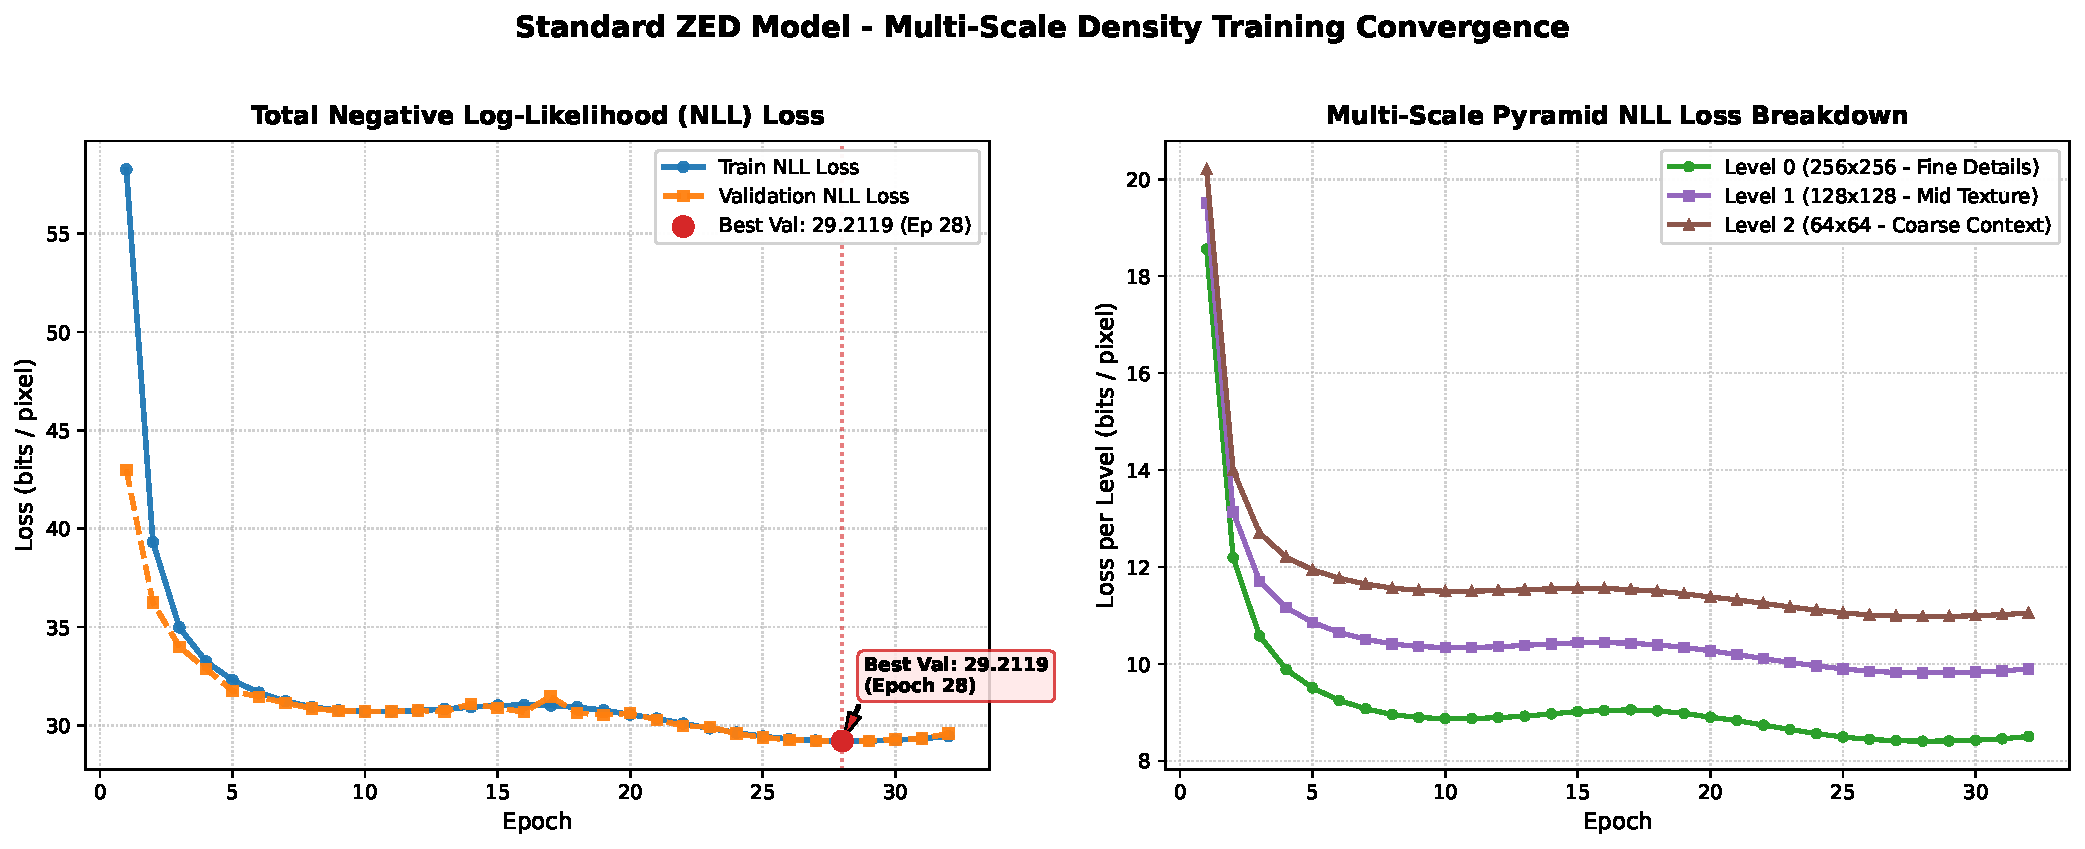
\includegraphics[width=\linewidth,height=0.60\textheight,keepaspectratio]{figures/training_curves_merged.pdf}\\[0.08em]
      \tiny\textcolor{SlateSub}{Đường cong hội tụ thực nghiệm: Train/Val loss và phân rã 3 cấp độ subpixel qua 32 epochs.}
    \end{column}
  \end{columns}
\end{frame}

% ==================== SLIDE 16: 6.2 CẤU HÌNH KIỂM ĐỊNH VÀ PHÂN TẦNG 70/30 ====================
\begin{frame}{6.2 Cấu hình kiểm định diện rộng \& Phân tầng 70/30}
  \framesubtitle{THỰC NGHIỆM ĐỘC LẬP \;\textbar\; INDEPENDENT EXPERIMENTAL EVALUATION}
  \begin{columns}[c, totalwidth=\linewidth]
    \begin{column}{0.44\linewidth}
      \begin{cleanbox}[top=0.4mm, bottom=0.4mm]{Tập dữ liệu kiểm định diện rộng}
        \raggedright\scriptsize
        \textbf{Tổng số lượng ảnh:} \textbf{179,042 ảnh}.\\
        \vspace{0.04em}
        \textbf{Ảnh thật tự nhiên:} \textbf{168,712 ảnh} (94.2\%).\\
        \vspace{0.04em}
        \textbf{Ảnh do AI sinh:} \textbf{10,330 ảnh} (5.8\%).\\
        \vspace{0.04em}
        \textbf{Mất cân bằng lớn:} Tỷ lệ $\sim$16:1 mô phỏng thực tế.
      \end{cleanbox}
      \vspace{0.06em}
      \begin{accentbox}[top=0.4mm, bottom=0.4mm]{TealAccent}{Phân tầng khoa học (Stratified Split)}
        \raggedright\tiny
        $\bullet$ \textbf{Tập Calibration (70\%):} 125,330 ảnh (118,099 thật + 7,231 AI) dùng tối ưu ngưỡng quyết định $\tau^*$.\\
        \vspace{0.04em}
        $\bullet$ \textbf{Tập Test ngoài mẫu (30\%):} 53,712 ảnh (50,613 thật + 3,099 AI) kiểm định độc lập với $\tau^*$ cố định.\\
        \vspace{0.04em}
        $\bullet$ \textbf{Phần cứng:} 2x Tesla T4 (DataParallel Kaggle).
      \end{accentbox}
    \end{column}
    \begin{column}{0.54\linewidth}
      \centering
      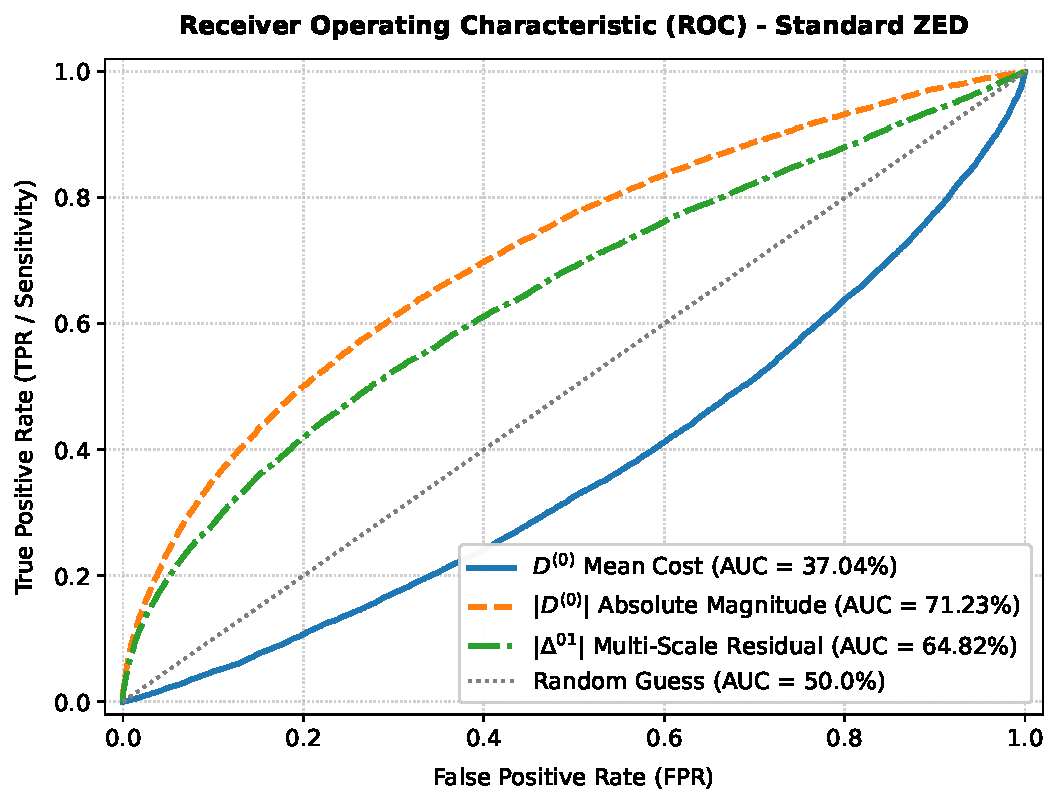
\includegraphics[width=\linewidth,height=0.58\textheight,keepaspectratio]{figures/roc_curves_comparison.pdf}\\[0.06em]
      \tiny\textcolor{SlateSub}{Đường cong ROC đa chỉ số trên tập Test độc lập (30\%).}
    \end{column}
  \end{columns}
\end{frame}

% ==================== SLIDE 17: 6.3 ĐÁNH GIÁ PHÂN TÁCH TRÊN TẬP TEST ====================
\begin{frame}{6.3 Đánh giá phân tách: So sánh hiệu năng trên tập Test (30\%)}
  \framesubtitle{THỰC NGHIỆM ĐỘC LẬP \;\textbar\; INDEPENDENT EXPERIMENTAL EVALUATION}
  \begin{columns}[c, onlytextwidth]
    \begin{column}{0.44\textwidth}
      % 2 ô KPI Stat Card
      \noindent\begin{minipage}[t]{0.48\linewidth}
        \begin{statbox}{ElectricBlue}{KPI 1}
          {\fontsize{13}{15}\selectfont\textbf{\textcolor{ElectricBlue}{68.76\%}}}\\[0.05em]
          {\tiny\textbf{\textcolor{MidnightNavy}{ROC-AUC $|D^{(0)}|$}}}
        \end{statbox}
      \end{minipage}\hfill
      \begin{minipage}[t]{0.48\linewidth}
        \begin{statbox}{EmeraldGreen}{KPI 2}
          {\fontsize{13}{15}\selectfont\textbf{\textcolor{EmeraldGreen}{64.01\%}}}\\[0.05em]
          {\tiny\textbf{\textcolor{MidnightNavy}{Balanced Acc}}}
        \end{statbox}
      \end{minipage}
      \vspace{0.15em}
      \begin{cleanbox}[top=0.8mm,bottom=0.8mm]{Bảng chỉ số kiểm định trên tập Test (30\%)}
        \centering\scriptsize
        \setlength{\tabcolsep}{1.6pt}
        \begin{tabular}{lcccc}
          \toprule
          \textbf{Chỉ số} & \textbf{ROC-AUC} & \textbf{Bal. Acc} & \textbf{Recall} & \textbf{Ngưỡng $\tau^*$} \\
          \midrule
          $D^{(0)}$        & 31.23\% & 50.01\% & 0.06\% & 3.707 \\
          \textbf{$|D^{(0)}|$} & \textbf{68.76\%} & \textbf{64.01\%} & \textbf{69.25\%} & \textbf{2.381} \\
          \textbf{$|\Delta^{01}|$} & \textbf{59.31\%} & \textbf{57.53\%} & \textbf{51.98\%} & \textbf{0.764} \\
          \bottomrule
        \end{tabular}
      \end{cleanbox}
      \vspace{0.15em}
      \begin{notebox}[top=0.8mm,bottom=0.8mm]
        \raggedright\tiny
        \textbf{Tính bền vững ngoài mẫu:}\\
        $|D^{(0)}|$ đạt Balanced Acc \textbf{64.01\%} trên tập Test độc lập (không suy giảm so với 63.78\% ở tập Calib), khẳng định tính tổng quát hóa không bị overfit.
      \end{notebox}
    \end{column}
    \begin{column}{0.54\textwidth}
      \centering
      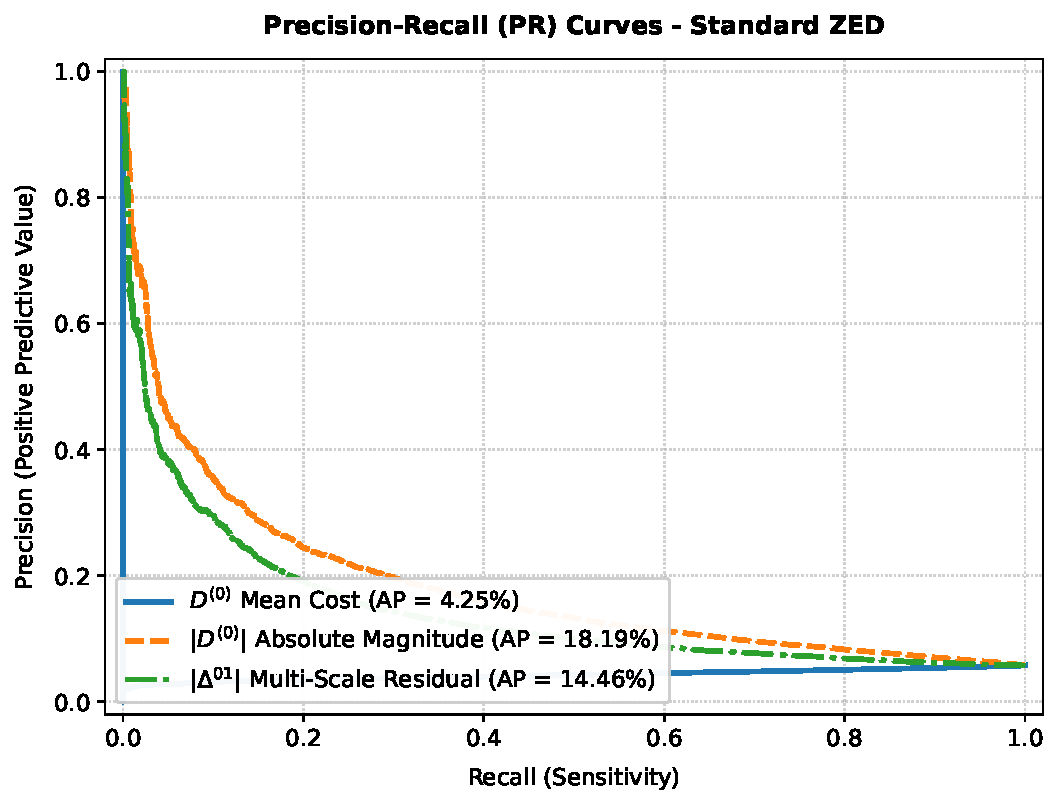
\includegraphics[width=\linewidth,height=0.62\textheight,keepaspectratio]{figures/pr_curves_comparison.pdf}\\[0.15em]
      \tiny\textcolor{SlateSub}{Đường cong PR: Khảo sát kịch bản mất cân bằng nghiêm trọng (16:1)}
    \end{column}
  \end{columns}
\end{frame}

% ==================== SLIDE 18: 6.4 PHÂN TÍCH CHỈ SỐ ĐỘT PHÁ |D^(0)| ====================
\begin{frame}{6.4 Phân tích chi tiết chỉ số đột phá $|D^{(0)}|$ trên tập Test}
  \framesubtitle{THỰC NGHIỆM ĐỘC LẬP \;\textbar\; INDEPENDENT EXPERIMENTAL EVALUATION}
  \begin{columns}[T, totalwidth=\linewidth]
    \begin{column}{0.31\linewidth}
      \vspace{0.05cm}
      \centering
      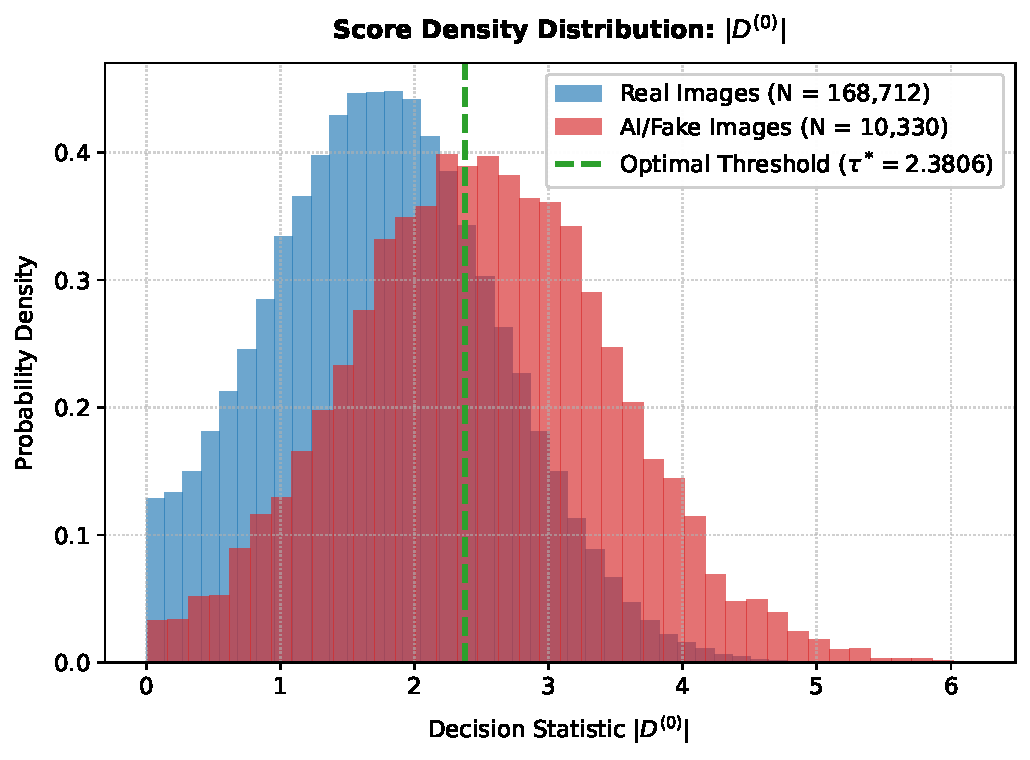
\includegraphics[width=\linewidth,height=0.41\textheight,keepaspectratio]{figures/density_abs_d0.pdf}\\[0.12em]
      \tiny\textcolor{SlateSub}{Score Density $|D^{(0)}|$ (Vạch ngưỡng $\tau^* = 2.381$)}
      \vspace{0.15em}
      \begin{notebox}[equal height group=s18box, top=0.8mm, bottom=0.8mm]
        \raggedright\tiny
        \textbf{Phân bố tách bạch:} Lấy trị tuyệt đối đưa phân phối ảnh AI dịch sang phải (mean cao hơn ảnh thật), tạo khoảng phân cách rõ rệt.
      \end{notebox}
    \end{column}
    \begin{column}{0.31\linewidth}
      \vspace{0.05cm}
      \centering
      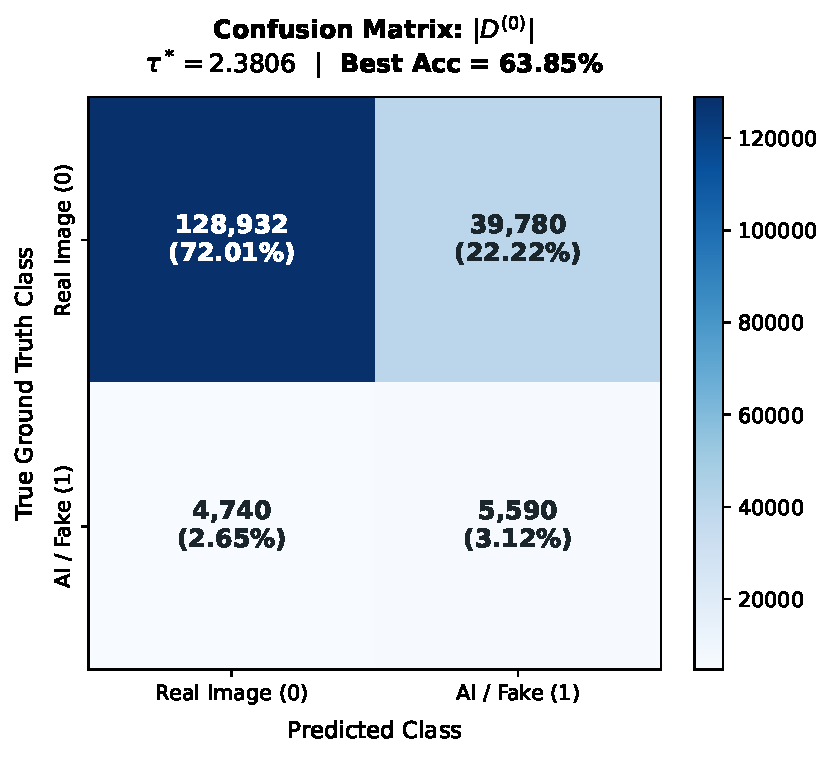
\includegraphics[width=\linewidth,height=0.41\textheight,keepaspectratio]{figures/confusion_matrix_abs_d0.pdf}\\[0.12em]
      \tiny\textcolor{SlateSub}{Confusion Matrix $|D^{(0)}|$ trên tập Test}
      \vspace{0.15em}
      \begin{notebox}[equal height group=s18box, top=0.8mm, bottom=0.8mm]
        \raggedright\tiny
        \textbf{Độ nhạy thực tế:} Phát hiện đúng \textbf{2,146 / 3,099 ảnh AI} (Recall 69.25\%) và nhận diện đúng 29,747 ảnh thật trên tập kiểm định ngoài mẫu.
      \end{notebox}
    \end{column}
    \begin{column}{0.35\linewidth}
      \vspace{0.05cm}
      \begin{accentbox}[top=1.5mm, bottom=1.5mm]{EmeraldGreen}{Ý nghĩa phương pháp \& Đột phá}
        \raggedright\tiny
        \textbf{1. Cơ chế đối xứng 2 phía:}\\
        Khắc phục triệt để hiện tượng ảnh AI bị nén quá mức ($D^{(0)} < 0$), nâng ROC-AUC từ 31.23\% lên 68.76\%.
        \vspace{0.20em}

        \textbf{2. Khả năng phát hiện zero-shot:}\\
        Đạt độ nhạy gần 70\% trên ảnh AI hoàn toàn không cần học mẫu fake nào trong quá trình huấn luyện.
        \vspace{0.20em}

        \textbf{3. Minh chứng thực nghiệm cho paper gốc:}\\
        Kết quả kiểm định diện rộng 179k ảnh hoàn toàn nhất quán với các kết luận lý thuyết của Cozzolino et al.
      \end{accentbox}
    \end{column}
  \end{columns}
\end{frame}

% ==================== SLIDE 19: KẾT LUẬN ====================
\begin{frame}{Kết luận}
  \framesubtitle{TỔNG KẾT BÁO CÁO \;\textbar\; CONCLUSION}
  \begin{columns}[t]
    \begin{column}{0.50\textwidth}
      \begin{accentbox}[equal height group=conc]{ElectricBlue}{Đóng góp về phương pháp \& lý thuyết}
        \raggedright\scriptsize
        \textbf{1. Cầu nối nén lossless \& thị giác máy tính:}\\
        Vận dụng lý thuyết thông tin Shannon để chuyển hóa bài toán phát hiện ảnh AI thành bài toán đo độ lệch chi phí nén.
        \vspace{0.25em}

        \textbf{2. Khung tiếp cận one-class thuần túy:}\\
        Chỉ học phân phối chuẩn của ảnh tự nhiên, triệt tiêu phụ thuộc vào dữ liệu giả hay kiến trúc bộ sinh cụ thể.
        \vspace{0.25em}

        \textbf{3. Thống kê Coding Cost Gap:}\\
        Đề xuất $|D^{(0)}|$ và $|\Delta^{01}|$ mang ý nghĩa vật lý rõ ràng, phân tách mạnh mẽ giữa ảnh thật và ảnh máy sinh.
      \end{accentbox}
    \end{column}
    \begin{column}{0.50\textwidth}
      \begin{accentbox}[equal height group=conc]{TealAccent}{Ý nghĩa thực tiễn \& kết quả thực nghiệm}
        \raggedright\scriptsize
        \textbf{1. Năng lực zero-shot vượt bậc:}\\
        Cả paper gốc và thực nghiệm độc lập đều chứng minh ZED duy trì hiệu năng cao trên các mô hình sinh mới lạ.
        \vspace{0.25em}

        \textbf{2. Kiểm chứng quy mô lớn (179,042 ảnh):}\\
        Đánh giá phân tầng khoa học 70\% Calib / 30\% Test khẳng định tính ổn định ngoài mẫu (Balanced Acc 64.01\%, Recall 69.25\%).
        \vspace{0.25em}

        \textbf{3. Khả thi trong triển khai thực tế:}\\
        Hệ thống không cần liên tục fine-tune khi xuất hiện các bộ sinh AI mới, mở ra giải pháp bền vững cho an toàn thông tin thị giác.
      \end{accentbox}
    \end{column}
  \end{columns}
\end{frame}

\end{document}
